\chapter{Diseño e Implementación} % Main chapter title

\label{Chapter3} % Change X to a consecutive number; for referencing this chapter elsewhere, use \ref{ChapterX}

\definecolor{mygreen}{rgb}{0,0.6,0}
\definecolor{mygray}{rgb}{0.5,0.5,0.5}
\definecolor{mymauve}{rgb}{0.58,0,0.82}

%%%%%%%%%%%%%%%%%%%%%%%%%%%%%%%%%%%%%%%%%%%%%%%%%%%%%%%%%%%%%%%%%%%%%%%%%%%%%
% parámetros para configurar el formato del código en los entornos lstlisting
%%%%%%%%%%%%%%%%%%%%%%%%%%%%%%%%%%%%%%%%%%%%%%%%%%%%%%%%%%%%%%%%%%%%%%%%%%%%%
\lstset{ %
  backgroundcolor=\color{white},   % choose the background color; you must add \usepackage{color} or \usepackage{xcolor}
  basicstyle=\footnotesize,        % the size of the fonts that are used for the code
  breakatwhitespace=false,         % sets if automatic breaks should only happen at whitespace
  breaklines=true,                 % sets automatic line breaking
  captionpos=b,                    % sets the caption-position to bottom
  commentstyle=\color{mygreen},    % comment style
  deletekeywords={...},            % if you want to delete keywords from the given language
  %escapeinside={\%*}{*)},          % if you want to add LaTeX within your code
  %extendedchars=true,              % lets you use non-ASCII characters; for 8-bits encodings only, does not work with UTF-8
  %frame=single,	                % adds a frame around the code
  keepspaces=true,                 % keeps spaces in text, useful for keeping indentation of code (possibly needs columns=flexible)
  keywordstyle=\color{blue},       % keyword style
  language=[ANSI]C,                % the language of the code
  %otherkeywords={*,...},           % if you want to add more keywords to the set
  numbers=left,                    % where to put the line-numbers; possible values are (none, left, right)
  numbersep=5pt,                   % how far the line-numbers are from the code
  numberstyle=\tiny\color{mygray}, % the style that is used for the line-numbers
  rulecolor=\color{black},         % if not set, the frame-color may be changed on line-breaks within not-black text (e.g. comments (green here))
  showspaces=false,                % show spaces everywhere adding particular underscores; it overrides 'showstringspaces'
  showstringspaces=false,          % underline spaces within strings only
  showtabs=false,                  % show tabs within strings adding particular underscores
  stepnumber=1,                    % the step between two line-numbers. If it's 1, each line will be numbered
  stringstyle=\color{mymauve},     % string literal style
  tabsize=2,	                   % sets default tabsize to 2 spaces
  title=\lstname,                  % show the filename of files included with \lstinputlisting; also try caption instead of title
  morecomment=[s]{/*}{*/}
}

En este capítulo se presentan las decisiones de diseño adoptadas para concretar el desarrollo del trabajo. Además, se describen en forma genérica los módulos necesarios tanto del sistema de enclavamiento como de los bloques auxiliares para concretar una comunicación exitosa entre el sistema y el exterior.

\section{Analizador de redes ferroviarias}

	En el marco de la Especialización de Sistemas Embebidos se utilizó el enfoque funcional basado en la tabla de enclavamientos, con las limitaciones ya expuesta en el capítulo 2. Algunos de los artículos encontrados utilizan ese enfoque \cite{Fun_1,Fun_2,Fun_3,Fun_4}, mientras otros artículos mas recientes abordan el modelado de los sistemas sin utilizar tablas de enclavamiento \cite{Geo_1,Geo_2,Geo_3,Geo_4}.
	
	Los diversos artículos que modelan los sistemas ferroviarios en base a la topología utilizan estrategias muy dispares. Por ejemplo, no existe una idea en común de que herramienta matemática utilizar: algunos recurren a las redes de Petri, mientras que otros a los grafos. Incluso dentro del subgrupo de los artículos que sugieren utilizar grafos no existe un criterio unificado de qué representa cada nodo y cada arista, ni tampoco cómo analizar la red ni cuáles son los elementos básicos que necesita para estar definida.	
	
	En base a la bibliografía relevada, se llegó a la conclusión de que todo grafo ferroviario necesita dos datos para estar definido. El primero es la lista de relaciones entre nodo inicial y nodo final, y el segundo es la posición absoluta del nodo en el grafo junto con datos adicionales, como si posee un paso a nivel o si es bidireccional. 
	
	Con esa información fue posible realizar un analizador de redes ferroviarias. Un script implementado en el lenguaje Python que procesa archivos de texto plano donde se indican las conexiones entre ellos y cuyos resultados son:
	
	\begin{itemize}
		\item Análisis de red ferroviaria:
		\begin{itemize}
			\item Determina qué cantidad de semáforos son necesarios.
			\item Determina dónde deben situarse los semáforos.
			\item Determina cuántos aspectos deben tener cada semáforo.
			\item Determina qué orientación debe tener cada semáforo.
			\item Identifica todos las máquinas de cambios.
			\item Identifica los extremos de la red, sean absolutos o relativos.
			\item Identifica todas las rutas soportadas por la red.
			\item Genera una tabla de enclavamientos con todos los datos obtenidos.
		\end{itemize}
		\item Implementación de la red ferroviaria en VHDL:
		\begin{itemize}
			\item Genera todos los archivos necesarios.
			\item Interconecta todos los módulos creados.
			\item Adapta el tamaño de todas las señales a lo que la topología necesite.
		\end{itemize}
		\item Interfaz de comunicación con la red ferroviaria:
		\begin{itemize}
			\item Genera todos las tramas necesarias para la comunicación.
			\item Brinda un menú de opciones para modificar las tramas en tiempo real.
			\item Envía las tramas al sistema implementado en la FPGA.
			\item Actualiza la interfaz con los datos devueltos por la FPGA.
		\end{itemize}
	\end{itemize}
	
	Todas las topologías de la sección \ref{Topologias} pueden ser analizadas por el programa y generar, de forma automática, el código en VHDL que sea necesario para el correcto funcionamiento del sistema. A modo de ejemplo se incluye el caso de la figura \ref{fig:Mapa_2_B}, grafo de una red ferroviaria bypass, antes de ser procesado. El analizador de redes ferroviarias devuelve el grafo procesado tal como se presenta en la figura \ref{fig:Mapa_2}.

	\begin{figure}[h]
	\centering
		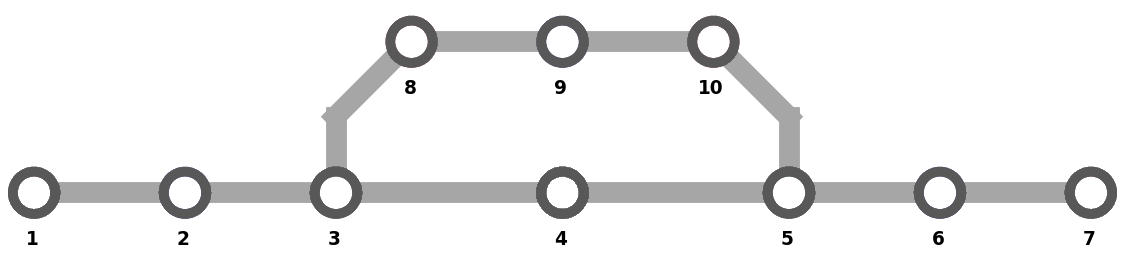
\includegraphics[scale=.4]{./Figures/Mapa_2_B}
		\caption{Grafo antes de ser analizado por el algoritmo}
		\label{fig:Mapa_2_B}
	\end{figure}
	
	\begin{figure}[h]
	\centering
		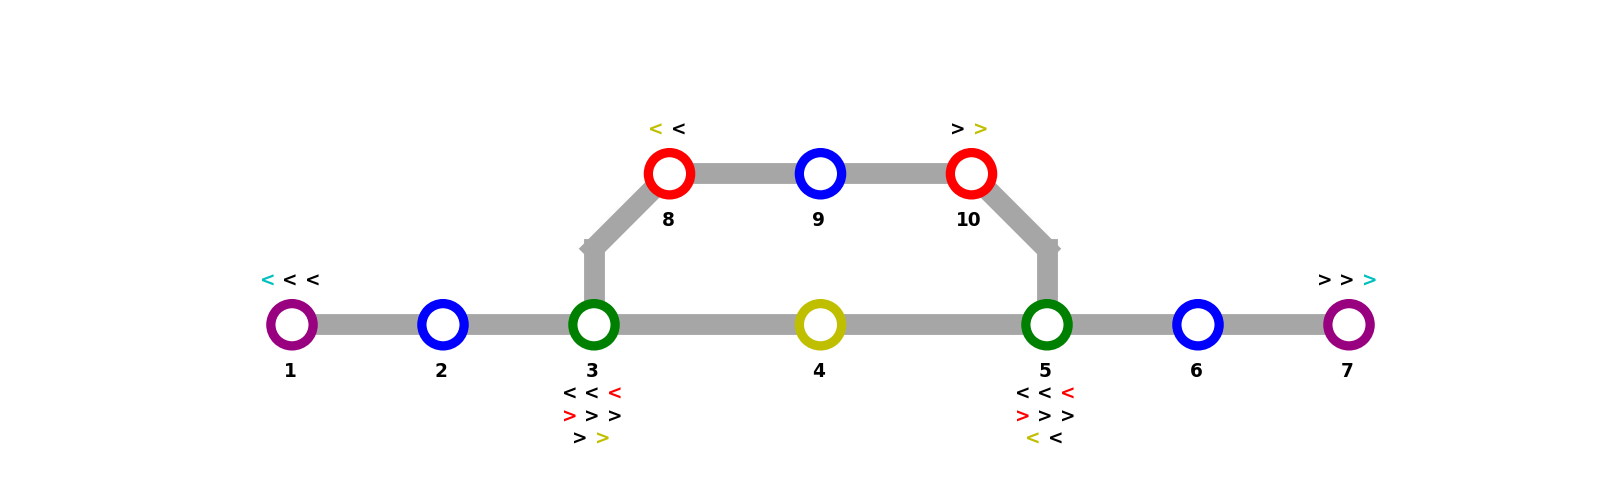
\includegraphics[scale=.4]{./Figures/Mapa_2}
		\caption{Grafo luego de ser analizado por el algoritmo}
		\label{fig:Mapa_2}
	\end{figure}		

	Los nodos 1 y 7 se encuentran pintados de violeta porque, al tener un único vecino cada uno, se consideran nodos extremos. Los nodos 2, 6 y 9 no presentan nada en especial, por lo que son nodos simples y están pintados de azul. Los nodos que sí tienen una importancia central en el análisis son los nodos que poseen tres vecinos: el nodo 3 y el nodo 5, que están pintados en verde y se consideran ''cambios raíz".

	Luego el nodo 4 se categoriza como nodo de cambio directo por ser la continuación de los segmentos 2-3 y 5-6 de tener el cambio de vía en posición normal, permitiendo la circulación directa. En este caso el nodo 4 es compartido por ambos cambios.
	
	Los nodos 8 y 10 son vecinos de los cambios 3 y 5 pero no comparten ninguna coordenada espacial con ellos, son nodos de cambios ramificados. Es decir, solo permitirán la secuencia de nodos 2-3-8 o 9-8-3 si la máquina de cambios se encuentra en posición inversa. El mismo análisis puede hacerse para el nodo 5.

	La asignación de semáforos se realiza solo sobre los nodos extremos, cambios raíz y cambios ramificados. Los extremos necesitan los semáforos para permitir la salida de las formaciones de la red, ya que la red ferroviaria continúa mas allá del nodo 1 y del 7; de ser nodos extremos absolutos (fin de red) no corresponde que se les asigne un semáforo.
	
	Los nodos de cambios son los que presentan mayor cantidad de semáforos. Necesitan dos semáforos de tres aspectos para permitir la circulación directa sobre el cambio cuando se encuentra en posición normal y un semáforo de dos aspectos para permitir la circulación en la ramificación del recorrido, pero con precaución por ser una zona crítica. Por último, los nodos de cambios ramificados solo presentan un semáforo de doble aspecto como complemento al otro semáforo de maniobras, en función de utilizar la ramificación para volver al recorrido principal a una velocidad moderada.
	
	El haber desarrollado un criterio propio para modelar las topologías tuvo como consecuencia el tener que diseñar tanto la herramienta de análisis, como así también la arquitectura y funcionalidad de cada uno de los módulos expuestos a continuación.	
	
\section{Módulo de nodos}
\label{nodos}
	El módulo de nodos corresponde al módulo principal en esta implementación. Por cada nodo en el grafo se tiene un módulo de nodos equivalente, cuyas conexiones a otros módulos estarán definidas por las aristas del grafo.
	
	Tal como se explicó en la sección \ref{grafos}, se definió que cada nodo del grafo representa un tramo de vía, con todos los elementos que posea ese tramo en la realidad. Es decir, si el tramo incluye semáforos o barreras serán modeladas dentro del módulo de nodo. Con excepción de las máquinas de cambios que por su naturaleza tendrán un módulo aparte.	
	
	Como cada tramo puede tener diferentes cantidades de elementos, existen diversos tipos de nodos en el sistema. Para ejemplificar se describirá el funcionamiento de un nodo genérico con la máxima cantidad de funcionalidades, de forma tal de cubrir todos los casos.
	
	Un módulo de nodo (cuyo diagrama de bloques se presenta en la figura \ref{fig:FSMD_Nodo}) recibe los estados de ocupación de sus vecinos (''Estado\_post\_i'' y ''Estado\_ante\_i'') y de sí mismo (''Estado\_i'') desde el exterior, además del estado de los semáforos que posee(''Sem\_s\_i[N\_SEM]''). 
	
	\begin{figure}[h]
	\centering
	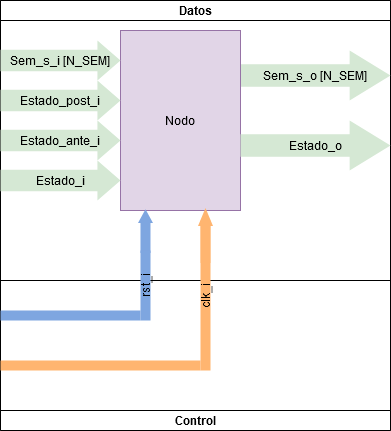
\includegraphics[scale=.5]{./Figures/FSMD-Nodo}
		\caption{Diagrama en bloques del módulo de nodo genérico}
		\label{fig:FSMD_Nodo}
	\end{figure}		
	
	%\vspace{10cm}
	
	Internamente debe informar su estado de ocupación a sus vecinos (''Estado\_o'') y decidir los aspectos que deben tener sus semáforos (''Sem\_s\_o[N\_SEM]'') de la siguiente manera:
			
	\begin{itemize}
		\item Si el tramo propio está ocupado: el semáforo propio debe estar en aspecto rojo.
		\item Si el vecino está ocupado: el semáforo propio debe estar en aspecto rojo.
		\item Si el vecino está desocupado:
		\begin{itemize}
			\item Si el semáforo vecino está en rojo: el semáforo analizado debe estar en aspecto amarillo.
			\item Si el semáforo vecino está en amarillo:  el semáforo analizado debe estar en aspecto verde.
		\end{itemize}				 
	\end{itemize}
	
\section{Módulo de la máquina de cambios}

	Una decisión de diseño importante fue que, a pesar de que los nodos del grafo pueden tener desde uno hasta seis vecinos, los módulos de nodos solo tienen dos posibles vecinos: el anterior y el posterior. Esto se hizo para que todos los nodos pudiesen ser modelados desde la misma plantilla base, agilizando la automatización del proceso.
	
	Esto llevó a la necesidad de disponer de un módulo que conmute las conexiones en el caso de tener nodos con mas de dos vecinos. Este bloque es el módulo de la máquina de cambios.
	
	Un cambio de vías conecta un tramo A con un tramo B o con un tramo C. El módulo de la máquina de cambios tiene como función conectar un nodo anterior (A) con un nodo posterior (B) o un nodo del desvío (C), según la posición de la máquina de cambios, como se muestra en la figura \ref{fig:Cambio_conexion}.
	
	\begin{figure}[h]
	\centering
	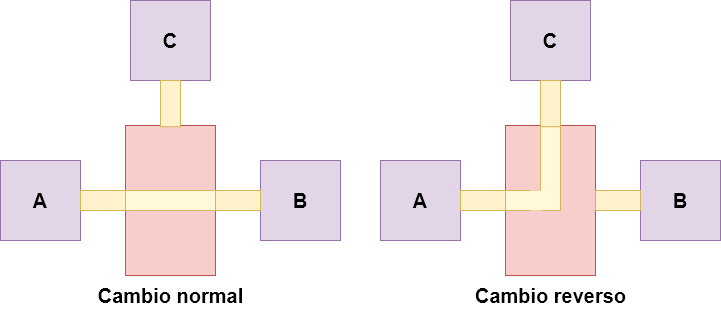
\includegraphics[scale=.5]{./Figures/FSMD-Conexiones}
		\caption{Conexión del módulo de la máquina de cambios}
		\label{fig:Cambio_conexion}
	\end{figure}	
	
	De esta manera, el nodo A ejemplificado en la figura \ref{fig:Cambio_conexion} tendrá como vecino posterior al que le indique la máquina de cambios. Si la posición del cambio es normal, entonces el nodo A tendrá como vecino posterior al nodo B. Si la posición del cambio es reversa, entonces el nodo A tendrá como vecino posterior al nodo C.
	
	De la misma manera los nodos B y C verán como nodo ''anterior'' al nodo A o a ningún nodo, según el cambio se encuentre en posición normal o reversa respectivamente.	
	
	En la figura \ref{fig:FSMD_Cambio} se ilustra el diagrama en bloques del módulo de la máquina de cambios.
	
	\begin{figure}[h]
	\centering
	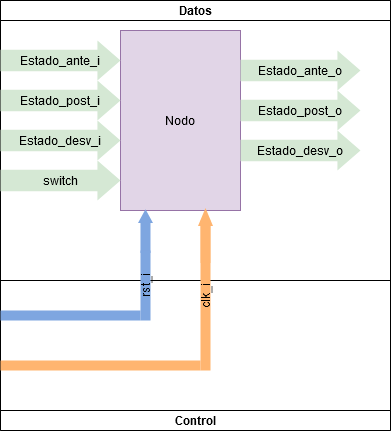
\includegraphics[scale=.5]{./Figures/FSMD-Cambio}
		\caption{Diagrama en bloques del módulo de máquina de cambios}
		\label{fig:FSMD_Cambio}
	\end{figure}
		
\section{Módulos de procesamiento de tramas}

	Durante el desarrollo del trabajo de la Especialización en Sistemas Embebidos se había considerado la estrategia de obtener las señales de forma paralela, es decir, para cada elemento se tenía asignado un pin que monitoreaba su estado. Esto resultó ser un problema a la hora de implementar topologías mas grandes, donde se necesitó hasta cinco veces la cantidad de entradas digitales que la FPGA tenía disponibles. Por lo tanto, se decidió cambiar a una lectura y escritura en serie.
	
	Sin embargo, utilizar una lectura serie implica que debe indicarse cuál es el inicio y el final de cada mensaje, además de un criterio para determinar si el mensaje recibido es fiable. La solución desarrollada se presenta a continuación en esta sección.
	
	\subsection{Módulo detector}
	
		El módulo detector tiene como función recibir una secuencia de caracteres y armar una salida con un vector de elementos booleanos. Un diagrama en bloques del funcionamiento del módulo se muestra en la figura \ref{fig:FSMD_Detector}
		
		\begin{figure}[h]
		\centering
			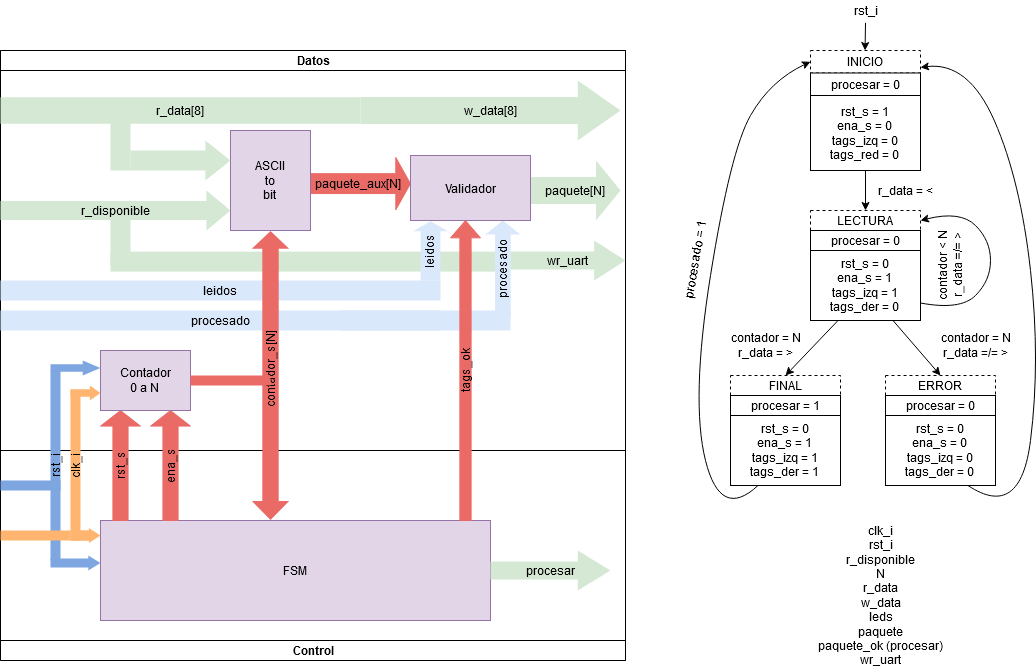
\includegraphics[scale=.6]{./Figures/FSMD-Detector}
			\caption{FSMD del módulo detector}
			\label{fig:FSMD_Detector}
		\end{figure}
		
		\vspace{10cm}
		
		La UART (del inglés, \textit{Universal Asynchronous Receiver-Transmitter}) es la unidad encargada de recibir y transmitir las tramas desde la computadora hasta la plataforma. Ésta envía secuencialmente un caracter por medio de la señal r\_data (8 bytes) y un pulso (r\_disponible) para informar que un nuevo dato ha sido enviado, además de indicar por medio de la señal N la cantidad de caracteres que serán enviados. 
		
		El proceso de detección se ilustra en la figura \ref{fig:Estados_Detector}.  		
		
		\begin{figure}[h]
		\centering
			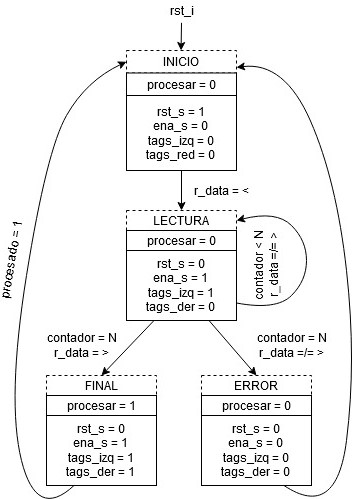
\includegraphics[scale=.65]{./Figures/Estados-Detector}
			\caption{Estados del módulo detector}
			\label{fig:Estados_Detector}
		\end{figure}
		
		%\vspace{10cm}
		
		En la figura \ref{fig:Estados_Detector} se tiene un estado inicial en el cual se espera el caracter de inicio de la trama ("$<$") que provoca una transición al estado de lectura. En dicho estado se recibirán hasta N caracteres mientras se actualiza un contador interno. Cuando el contador interno iguale la cantidad N, se verifica si el próximo caracter es el de fin de trama ("$>$").
		
		Si el caracter leído es el de final de trama, se pasa al estado final, donde el paquete es considerado válido y enviado a la próxima etapa junto con su pulso de validación del dato. Si el caracter leído es distinto, entonces se descarta toda la trama y se vuelve al inicio a la espera de otro caracter de inicio de trama, reiniciando todas las variables auxiliares.
		
		Internamente se tienen diversas variables auxiliares para controlar si se han recibido los delimitadores y si la cantidad recibida es correcta. Eso cobra gran importancia al realizar los ensayos, porque se puede diferenciar rápidamente la fuente de posibles errores.
		
	\subsection{Módulo registro}
	
		Así como el módulo de detección realiza una conversión de caracteres (1 byte) a booleanos (1 bit), el módulo de registro (figura \ref{fig:FSMD_Registro}) hace la operación inversa. Dado un vector de elementos booleanos, el módulo debe generar M caracteres '0' o '1' según corresponda en base al vector, y enviarlos a la UART para su posterior impresión.
		
		\begin{figure}[h]
		\centering
			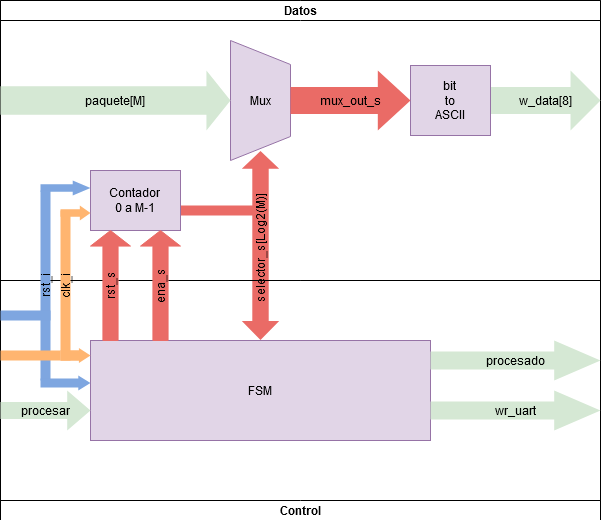
\includegraphics[scale=.65]{./Figures/FSMD-Registro}
			\caption{FSMD del módulo registro}
			\label{fig:FSMD_Registro}
		\end{figure}

		%\vspace{10cm}
		
		La máquina de estados (FSM) desarrollada se ocupa de generar cada dos ciclos de reloj un pulso para poder enviar secuencialmente los caracteres detectados. A la vez que el multiplexor va seleccionando cada elemento del vector paquete[M] según el valor del contador vigente, que se incrementa cada pulso del reloj interno generado.
		
		Finalmente se envía un caracter ASCII '1' si el elemento i-ésimo del paquete es '1' lógico y un "0" si lo recibido es un '0' lógico. Junto con el caracter se envía la señal ''wr\_uart'' para indicarle a la UART que ese dato debe ser guardado en una estructura de memoria llamada FIFO (del inglés, \textit{First-In,First-Out}) de salida y la señal ''procesado'' para indicarle al módulo de detección que ya puede recibir nuevas tramas.
	
		La máquina de estados se ilustra en la figura \ref{fig:Estado_Registro}. 
		
		\begin{figure}[h]
		\centering
			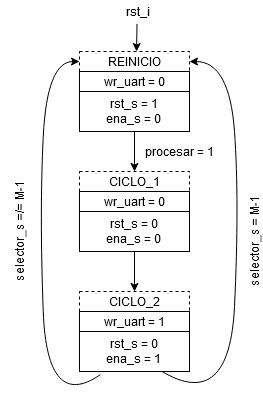
\includegraphics[scale=.85]{./Figures/Estados-Registro}
			\caption{Estados del módulo registro}
			\label{fig:Estado_Registro}
		\end{figure}
		
		\vspace{10cm}	
		
		Se añadieron dos estados para generar el pulso de reloj necesario para mantener sincronizadas las tramas. Al estado de reinicio se accede cuando el contador haya recorrido todos los elementos del paquete, igualando el valor de M, la cantidad de elementos esperados. 
		
		La señal ''procesar'' se recibe de las etapas anteriores. Si la trama ingresada es incorrecta, o si ya fue impresa, entonces esa señal será '0' y el registro dejará de enviar datos a la UART. En caso afirmativo (''procesar'' = '1') el proceso continuará hasta que la UART indique que no pueda recibir mas datos o que alguna etapa previa informe de algún error en el proceso.
		
	\subsection{Módulo selector}
	
		Para facilitar el proceso se añadió la posibilidad de elegir con uno de los switches del kit de desarrollo el puntear completamente el enclavamiento. En la figura \ref{fig:FSMD_Selector} se ilustra brevemente el módulo diseñado para lograr este objetivo.
		
		El módulo selector permite que ante un cambio en la posición del switch la salida sea una copia exacta de la entrada, lo cuál permitió diseñar todo el proceso de detección, lectura y escritura en la UART de forma independiente al enclavamiento. Mientras que con la otra posición del switch se enviaba la señal de entrada al sistema de enclavamiento y la salida era la consecuencia de haber pasado por este proceso.
		
		\begin{figure}[h]
		\centering
			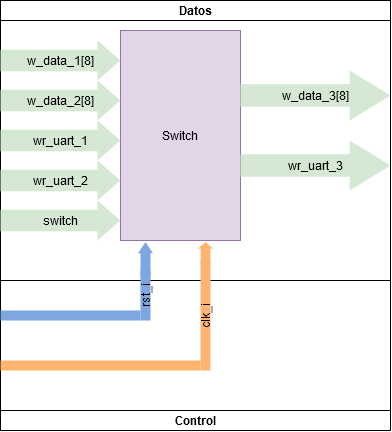
\includegraphics[scale=.6]{./Figures/FSMD-Selector}
			\caption{Diagrama de bloques del módulo selector}
			\label{fig:FSMD_Selector}
		\end{figure}	
		
		\vspace{10cm} 
		
		La implementación permite enviar la entrada a una salida u otra según la posición del switch, de forma asincrónica. Aunque no solo envía el dato sino también la ráfaga de pulsos asociada para su correcta escritura en la UART.
			
\section{Módulos de adaptación a enclavamiento}
	
	Para el modelo de los estados de las barreras, circuitos de vías y máquinas se cambios se adoptó la convención de la Tabla \ref{Bool_1}.
	
	\begin{table}[!hbt]
	\renewcommand{\arraystretch}{1.3}
	\caption{Convención para elementos ferroviarios I}
	\label{Bool_1}
	\centering
	\begin{tabular}{ c  c  c  c }
	\hline	
	Estado & Barrera & Máquina de cambiós & Circuito de vía \\	
	\hline
	'0' & Baja & Posición normal & Ocupado \\	
	'1' & Alta & Posición inversa & Desocupado \\	
	\hline
	\end{tabular}
	\end{table}	
	
	En el caso de los semáforos, dependiendo de la cantidad de aspectos, pueden tenerse tres o cuatro estados. Por lo tanto la convención que se definió es la que se muestra en la Tabla \ref{Bool_2}.
	
	\begin{table}[!hbt]
	\renewcommand{\arraystretch}{1.3}
	\caption{Convención para elementos ferroviarios II}
	\label{Bool_2}
	\centering
	\begin{tabular}{ c  c  c  c }
	\hline
	Estado & Semáforo [2 aspectos] & Semáforo [3 aspectos] & Semáforo [4 aspectos] \\	
	\hline
	'00' & Rojo & Rojo & Rojo \\	
	'01' & Amarillo & Amarillo & Amarillo \\	
	'10' & - & - & Doble amarillo \\
	'11' & - & Verde & Verde \\
	\hline
	\end{tabular}
	\end{table}	
	
	Queda de manifiesto que se pueden enviar tramas conformadas únicamente por ceros y unos de forma serializada a la plataforma FPGA. De esta manera, luego se podría procesar la trama e ir dividiendo cada porción de datos en información a la zona que le corresponda. 
	
	Una forma de organizar la trama de entrada fue la adoptada en la Tabla \ref{Trama_in}. En la misma, se envían en orden todos los estados de ocupación, seguidos de todos los estados de los semáforos (intercalando el bit mas significativo con el menos significativo), los estados de las barreras y finalmente los estados de las máquinas de cambios.
	
	\begin{table}[!hbt]
	\renewcommand{\arraystretch}{1.3}
	\caption{Trama de entrada [N]}
	\label{Trama_in}
	\centering
	\begin{tabular}{ | c | c | c | c | }
	\hline
	Ocupación & Semáforos & Barreras & Cambios \\
	\hline	
	\end{tabular}
	\end{table}		 
	
	La trama de salida se definió que sea muy similar, salvo que los estados de ocupación no serán un dato a transmitir ya que son de solo lectura y se asume que el mismo no ha cambiado durante el tiempo de procesamiento. La trama se definió en la Tabla \ref{Trama_out}.
	
	\begin{table}[!hbt]
	\renewcommand{\arraystretch}{1.3}
	\caption{Trama de salida [M]}
	\label{Trama_out}
	\centering
	\begin{tabular}{| c | c | c | }
	\hline
	  Semáforos & Barreras & Cambios \\
	\hline	
	\end{tabular}
	\end{table}	
	
	El módulo de enclavamientos espera como entradas las señales de estado de cada elemento en paralelo. Pero, como ya se definió en las Tablas \ref{Trama_in} y \ref{Trama_out}, la entrada del sistema es serializada. Por lo tanto, es necesario tener dos módulos que adapten ambas etapas: 
	
	\begin{itemize}
		\item Módulo separador: encargado de convertir las entradas seriales en señales en paralelo y distribuir los datos según donde sean requeridos.
		\item Módulo mediador: encargado de serializar las señales en paralelo que genera el enclavamiento, según el orden requerido.
	\end{itemize}
	 
	\subsection{Módulo separador}
	
		El módulo separador diseñado se puede ver en la figura \ref{fig:FSMD_Separador}. Este debe recibir el vector de elementos booleanos de tamaño N (''paquete[N]'') y la orden de que debe procesarlo (''procesar''). 
		
		\begin{figure}[h]
		\centering
			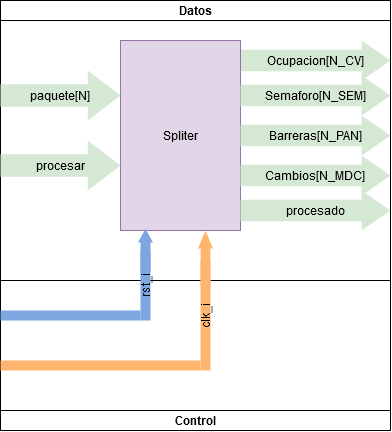
\includegraphics[scale=.5]{./Figures/FSMD-Separador}
			\caption{Diagrama de bloques del módulo separador}
			\label{fig:FSMD_Separador}
		\end{figure}
		
		\vspace{7cm}
		
		A continuación, como el generador de código sabe previamente la cantidad de cada uno de los elementos ferroviarios, puede descomponer los elementos del vector paquete[N] en vectores mas pequeños según corresponda.
		
	\subsection{Módulo mediador}
	
		El módulo mediador diseñado, que se puede visualizar en la figura \ref{fig:FSMD_Mediador}, tiene como función volver a generar el vector de elementos booleanos que ya han sido procesados por el enclavamiento.
		
		\begin{figure}[hbt]
		\centering
			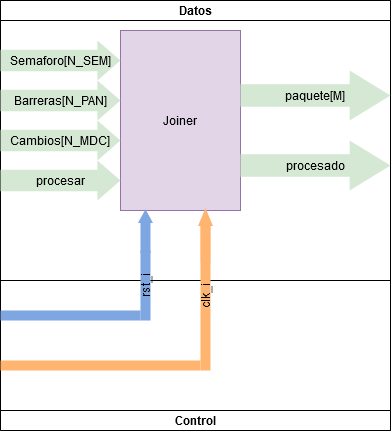
\includegraphics[scale=.48]{./Figures/FSMD-Mediador}
			\caption{Diagrama de bloques del módulo mediador}
			\label{fig:FSMD_Mediador}
		\end{figure}
		
		\vspace{10cm}
		
		El módulo mediador recibe la salida del enclavamiento y la orden de generar el paquete (''procesar''). Una vez que el vector (''paquete[M]'') ha sido creado, se envía una variable de control ("procesado") a la siguiente etapa para poder coordinar todo el sistema con un solo reloj.


		
\section{Módulo de comunicación UART}

	En el diseño de los módulos para la interface UART con el exterior se utilizó un modelo  aportado por los docentes, pero fue necesario modificarlo para poder automatizarlo y cumplir con las siguientes premisas:
	
	\begin{itemize}
		\item Se deben tener dos FIFOs distintas, una de entrada y la otra de salida.
		\item El tamaño de las FIFOs debe adaptarse a la topología: redes mas grandes necesitarán FIFOs mas grandes y redes mas pequeñas requerirán FIFOs mas pequeñas.
		\item Ambas FIFOS no pueden tener tamaño idéntico.
		\item Se deben incluir señales que indiquen al sistema si se tienen nuevos datos del exterior o si es posible recibir nuevos datos procesados para su posterior impresión.
		\item Cada cierto tiempo ambas FIFOS deberán vaciarse en su totalidad.		
	\end{itemize}
	
		Se presenta en la figura \ref{fig:FSMD_UART} un diagrama en bloques de la UART.
			
		\begin{figure}[h]
		\centering
		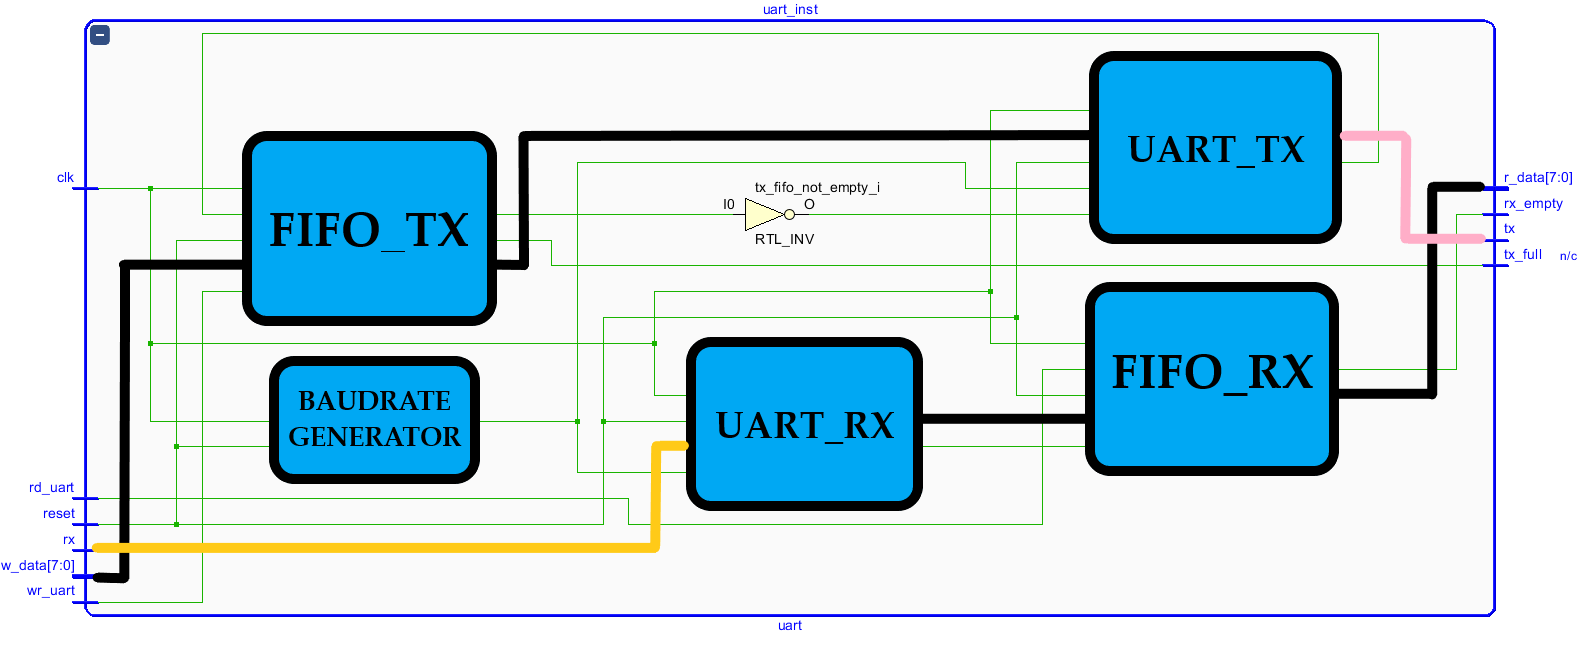
\includegraphics[scale=.35]{./Figures/UART}
			\caption{Diagrama en bloques de la UART}
			\label{fig:FSMD_UART}
		\end{figure}

		Los bloques de recepción y transmisión son funcionalmente idénticos, pero instanciados de forma diferente para que adopten tamaños distintos y sean conectados a señales distintas, ya que su rol no es el mismo. La FIFO de entrada es la encargada de almacenar los valores ingresados (conector amarillo) en la plataforma con un \textit{baud-rate} definido y envía su contenido al sistema junto con una serie de pulsos para indicar cuándo deben ser leídos. La FIFO de salida, en cambio, debe almacenar los resultados del sistema según una serie de pulsos generada por el mismo sistema, para luego imprimir el resultado por el puerto serie (conector rosa) con el \textit{baud-rate} definido.

		La FIFO de entrada se utiliza para almacenar una trama de la forma '<Mensaje de largo N>' (conector negro) por lo que espera al menos N+2 bytes, mientras que la FIFO de salida espera mensajes de la forma 'Mensaje de largo M' (conector negro). Ya que N > M es claro que N + 2 > M en la mayoría de los casos. Aunque también puede ocurrir que la diferencia entre ambos no sea tanta y al implementar el tamaño de las FIFOs en potencias de 2 terminen ambas FIFOs con el mismo tamaño. 

		Con este criterio de diseño, en todos los demás casos, la FIFO de salida tendrá el mismo tamaño que la FIFO de entrada o a lo sumo será $50$\% menor, lo que representa un ahorro de $25$\% de los recursos estimados. Por ejemplo, si se necesita que la entrada tenga 15 elementos y la salida 7 elementos y se le asigna el mismo tamaño a ambas FIFOs; tanto la FIFO de entrada como la de salida necesitarán 16 bits cada una, dando un total de 32 bits. Pero si se aplica el criterio de tamaños desacoplados, entonces para la FIFO de salida podrían asignarse solamente 8 bits, dando un total de 24 bits, un $25$\% menos que los 32 bits que necesitaría si ambas FIFOs quedaran definidas según los datos de la entrada.
		
\section{Interfaz de comunicación Python}

	El algoritmo analizador de redes ejecuta la conexión de la consola utilizada con la plataforma FPGA. Presenta al usuario un menú de opciones para ocupar/desocupar ciertos tramos de la vía, cambiar el aspecto de ciertos semáforos, pedir que una barrera suba o baje o incluso modificar la posición de una máquina de cambios.
	
	En la figura \ref{fig:Menu_UART} se ilustra el menú diseñado para ingresar los comandos al sistema. Ya que existe una interfaz mucho mas avanzada desarrollada por otra parte del equipo de investigación en UTN Haedo, no se ha invertido demasiado tiempo en tener una interfaz propia para realizar pruebas a mayor escala.
	
		\begin{figure}[h]
		\centering
		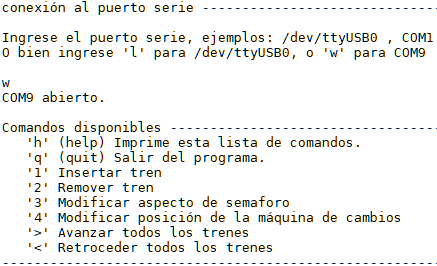
\includegraphics[scale=.76]{./Figures/Test/UART_2}
			\caption{Menú de opciones para comunicarse con el sistema-}
			\label{fig:Menu_UART}
		\end{figure}
	
	\vspace{5cm}
	
	Todos los cambios repercuten en el grafo mostrado en pantalla (figura \ref{fig:Grafo_UART}), que cambiará los colores de los semáforos y de los nodos para representar la ocupación del tren; así como también el color de las aristas para indicar la posición de los cambios.
	
		\begin{figure}[h]
		\centering
		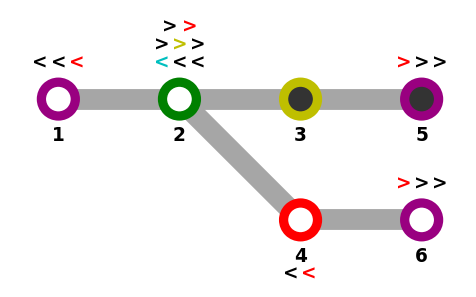
\includegraphics[scale=.76]{./Figures/Mapa_interfaz}
			\caption{Grafo modificado en tiempo real por la FPGA.}
			\label{fig:Grafo_UART}
		\end{figure}

	De esta forma es posible simular el comportamiento de toda la topología: posición de cada semáforo, aspectos de las señales y su orientación, clasificación de cada nodo, posición de las máquinas de cambios, etc. Esto permite verificar con mayor facilidad que el comportamiento sea el esperado.

	En el siguiente capítulo se presentarán los ensayos y resultados que permiten analizar el funcionamiento del proceso automatizado de implementación desarrollado.
